% Author: Izaak Neutelings (Februari, 2020)
% http://texample.net/tikz/examples/tag/circuitikz/
% http://texample.net/tikz/examples/circuitikz/
% https://www.overleaf.com/learn/latex/CircuiTikz_package
% http://texdoc.net/texmf-dist/doc/latex/circuitikz/circuitikzmanual.pdf
% http://repositorios.cpai.unb.br/ctan/graphics/pgf/contrib/circuitikz/circuitikzmanual.pdf
\documentclass[border=3pt,tikz]{standalone}
\usepackage{amsmath} % for \dfrac
\usepackage{physics}
\usepackage{tikz,pgfplots}
\usepackage[siunitx]{circuitikz} %[symbols]
\usepackage[outline]{contour} % glow around text
\usetikzlibrary{arrows,arrows.meta}
\usetikzlibrary{decorations.markings}
\tikzset{>=latex} % for LaTeX arrow head
\usepackage{xcolor}
\colorlet{Icol}{blue!50!black}
\colorlet{Ccol}{orange!90!black}
\colorlet{Rcol}{green!50!black}
\colorlet{Lcol}{blue!50!black}
\colorlet{loopcol}{red!90!black!25}
\colorlet{pluscol}{red!60!black}
\colorlet{minuscol}{blue!60!black}

\ctikzset{bipoles/generic/width=1.2, bipoles/generic/height=0.5}



\begin{document}


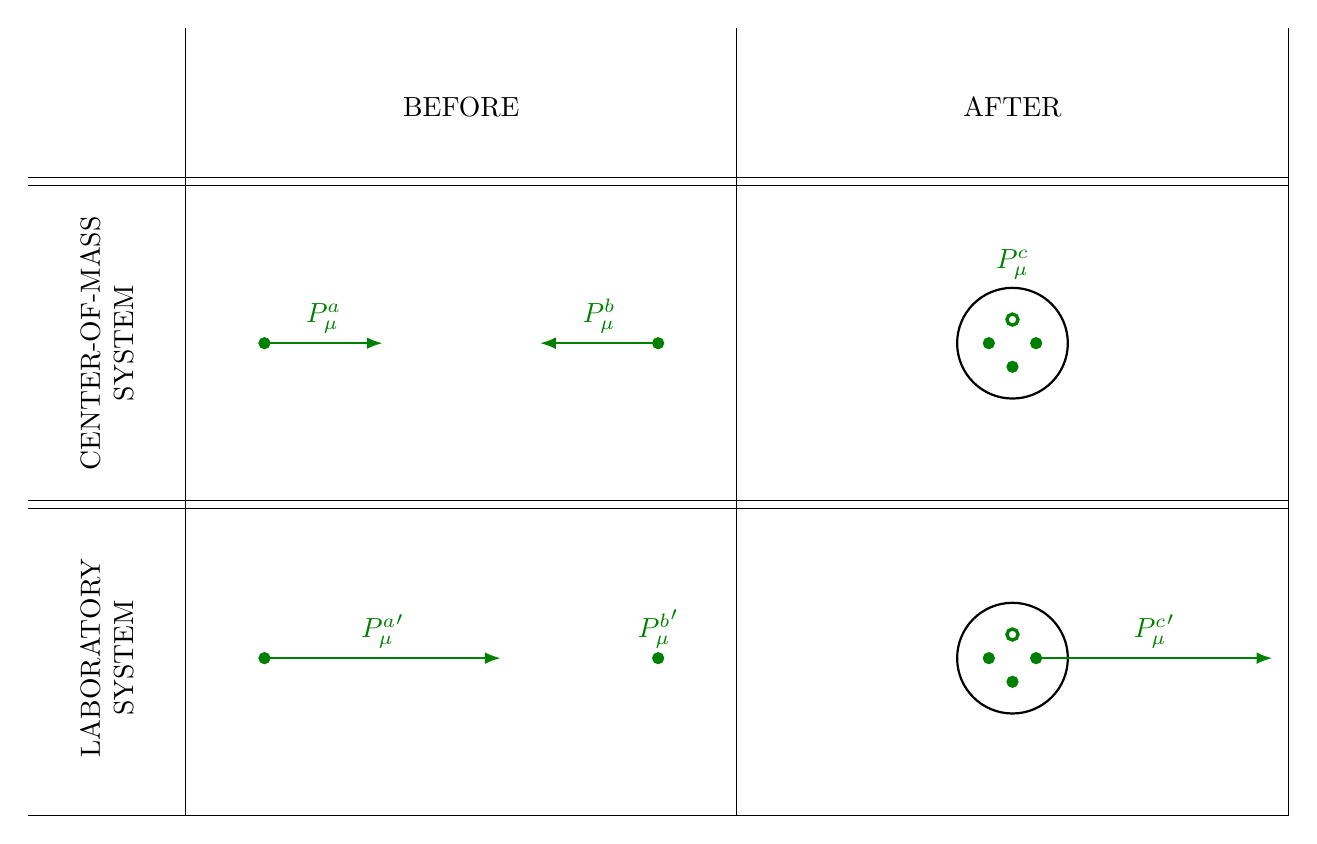
\begin{tikzpicture}[]

    

    % \draw[-{Latex[length=2mm]}, dashed, thick, bend left=10, Rcol] ( axis cs:6.2, -0.4) node [right] {$5.52$} to (axis cs:5.52, 0);

    \draw[] (-3, 2) -- (13, 2);
    \draw[] (-3, 2.1) -- (13, 2.1);
    \draw[] (-1, 4) -- (-1, -6);
    \draw[] (6, 4) -- (6, -6);
    \draw[] (13, 4) -- (13, -6);
    \draw[] (-3, -2) -- (13, -2);
    \draw[] (-3, -2.1) -- (13, -2.1);
    \draw[] (-3, -6) -- (13, -6);

    \node[] at (2.5, 3) {BEFORE};
    \node[] at (9.5, 3) {AFTER};

    \node[rotate=90, align=center] at (-2, 0) {CENTER-OF-MASS\\SYSTEM};
    \node[rotate=90, align=center] at (-2,-4) {LABORATORY\\SYSTEM};

    \filldraw[Rcol] (0, 0) circle (2pt);
    \filldraw[Rcol] (5, 0) circle (2pt);
    \draw[-{Latex[length=2mm]}, thick,  Rcol] (0, 0)  to node [midway, above] {$P^a_\mu$} (1.5, 0) ;
    \draw[-{Latex[length=2mm]}, thick,  Rcol] (5, 0)  to node [midway, above] {$P^b_\mu$}(3.5, 0) ;

    \filldraw[Rcol] (0, -4) circle (2pt);
    \filldraw[Rcol] (5, -4) circle (2pt);
    \draw[-{Latex[length=2mm]}, thick,  Rcol] (0, -4)  to node [midway, above] {${P^a_\mu}'$} (3, -4) ;

    \node[-{Latex[length=2mm]}, thick,  Rcol, above]  at (5, -4) {${P^b_\mu}'$};

    
    \draw[black, thick] (9.5, 0) circle (20pt);
    \filldraw[Rcol] {(9.5, 0) + (0.3, 0)} circle (2pt);
    \filldraw[Rcol] {(9.5, 0) + (-0.3, 0)} circle (2pt);
    \filldraw[Rcol] {(9.5, 0) + (0, -0.3)} circle (2pt);
    \draw[Rcol, very thick] {(9.5, 0) + (0, 0.3)} circle (2pt);
    \node[Rcol] at (9.5, 1) {$P^c_\mu$};
    
    \draw[black, thick] (9.5, -4) circle (20pt);
    \filldraw[Rcol] {(9.5, -4) + (0.3, 0)} circle (2pt);
    \filldraw[Rcol] {(9.5, -4) + (-0.3, 0)} circle (2pt);
    \filldraw[Rcol] {(9.5, -4) + (0, -0.3)} circle (2pt);
    \draw[Rcol, very thick] {(9.5, -4) + (0, 0.3)} circle (2pt);
    \draw[-{Latex[length=2mm]}, thick,  Rcol] (9.8, -4)  to node [midway, above] {${P^c_\mu}'$} (12.8, -4) ;

    
    % \coordinate (P1) at (0, 0);
    % \coordinate (P2) at (3, 0);
    % \coordinate (P3) at (3, -3.5);
    % \coordinate (P4) at (3, -7);
    % \coordinate (P5) at (0, -7);
    % \coordinate (P6) at (0, -4.5);
    % \coordinate (P7) at (0, -2.5);

    % \filldraw [black] (P1) circle (1.5pt);
    % \filldraw [black] (P2) circle (1.5pt);
    % \filldraw [black] (P3) circle (1.5pt);
    % \filldraw [black] (P4) circle (1.5pt);
    % \filldraw [black] (P5) circle (1.5pt);
    % \filldraw [black] (P6) circle (1.5pt);
    % \filldraw [black] (P7) circle (1.5pt);

    % \draw (P1) node[left, pluscol] {$a$} to[generic, name=g2] (P2) node [right, pluscol] {$b$};
    % \node at (g2.center) {$z_2$}; 

    % \draw[-{Latex[length=3mm]}, dashed, thick, bend left=-35] (P1) to node [midway, below] {$V_2$} (P2) ;

    % \draw (P2) to[generic, name=g3] (P3) node [right, pluscol] {$c$};
    % \node at (g3.center) {$z_3$}; 

    % \draw[-{Latex[length=3mm]}, dashed, thick, bend left=-35] (P2) to node [midway, left] {$V_3$} (P3) ;

    % \draw (P3) to[generic, name=g4] (P4) node [right, pluscol] {$d$};
    % \node at (g4.center) {$z_4$}; 

    % \draw[-{Latex[length=3mm]}, dashed, thick, bend left=-35] (P3) to node [midway, left] {$V_4$} (P4) ;

    % \draw (P4) to[generic, name=g5] (P5) node [left, pluscol] {$e$};
    % \node at (g5.center) {$z_5$}; 

    % \draw[-{Latex[length=3mm]}, dashed, thick, bend left=-35] (P4) to node [midway, above] {$V_5$} (P5) ;

    % \draw (P5) to[generic, name=g6] (P6) node [left, pluscol] {$f$};
    % \node at (g6.center) {$z_6$}; 

    % \draw[-{Latex[length=3mm]}, dashed, thick, bend left=-45] (P5) to node [midway, right] {$V_6$} (P6) ;

    % \draw (P6) -- (P7) node [left, pluscol] {$g$};
    % \filldraw[fill=white, thick] (0, -3.5) circle (15pt);
    % \draw[-{Latex[length=2mm]},  thick] (-0.2, -3.7) to node [midway, right, minuscol] {$\mathcal{E}$} (-0.2, -3.3); 

    % \draw[-{Latex[length=3mm]}, dashed, thick, bend left=-89] (P6) to node [midway, right] {$V_7$} (P7) ;

    % \draw (P7) to[generic, name=g1] (P1);
    % \node at (g1.center) {$z_1$}; 

    % \draw[-{Latex[length=3mm]}, dashed, thick, bend left=-45] (P7) to node [midway, right] {$V_1$} (P1) ;

    % \node [Icol, left] at (2, -4) {$\Gamma$};
    % \draw[-{Latex[length=2mm]}, Lcol, thick, bend left=45] (2, -4) to (2.5, -4.3) ;
    % \draw (-0.5, 0) to (-2, 0) to [thick L] (-2, 2) to[thick R] (2, 2) to [thick C] (2, 0) -- (0.5, 0); 

    % \draw[fill=white] (-0.5, 0) circle (2pt) node [yshift=-10] {$1$};
    % \draw[fill=white] (0.5, 0) circle (2pt) node [yshift=-10] {$2$};
    % \node [] (0, 0) {$V$};
    
\end{tikzpicture}

\end{document}